\subsection{\dmap Application}


%\begin{figure}[!htbp]
%    \centering
%    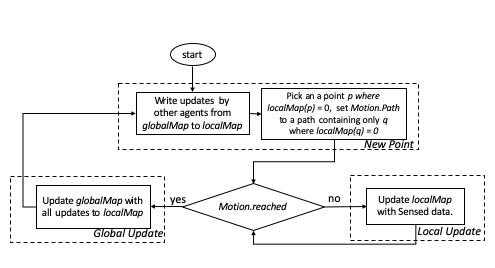
\includegraphics[width=\linewidth]{figs/map_flowchart.png}
%    \caption{Flowchart for a simple solution to 2D distributed mapping problem\vspace{-2mm}}
%    \label{fig:flowmap}
%\end{figure}



We discuss now discuss how our algorithm implemented $\lgname$ shown in \reffig{mapapp} tackles $\mapprob$. \reffig{flowmap} shows a simple idea for solving this problem for each robot:

The variable $\lmap$ refers to the current mapping $\map_i$ constructed by each robot $i$ using the algorithm. The function $\mathit{MaxExp}$ informally, determines whether there is a grid rectangle in the frontier of the current $\map_i$ . If not, the robot first updates its $\lmap$ from $\gmap$, which is used for sharing the currently computed occupancy maps by all robots so far. The robot then picks a new point in a rectangle known to be unoccupied in its $\lmap$ and follows a path ($\mathit{Motion.Path}$) moving only over grid rectangles known to be unoccupied by its $\lmap$. While the robot hasn't reached the target rectangle, it keeps updating its $\lmap$ with sensed data (occupied and unoccupied rectangles). When it reaches the target, it updates the $\gmap$ from its $\lmap$.

\sayan{Assumption about 
 \emph{rounds} of duration $\delta$, and in each round, each robot performs an action, which is expressed in $\lgname$ as an event.}


\subsection{Analysis of \dmap}
\label{sec:analysis}



Having defined the state of the robot, we now analyze the $\lgname$ program shown in \reffig{mapapp}. Given a robot $i$, ${\bf s}.\lmap_i$ represents the \emph{local} map, $\map_i$ constructed by each robot. $s_i.M.\gmap$ represents the \emph{global} map, $\map$ constructed from the local maps as outlined in \defn{cons}. In implementation, if $\map_i$ is not defined on $q\in Q$, then we set $\lmap[q] = -1$. Consequently, if $\map$ is not defined, we set $\gmap[q] = -1$.


We omit the initialization of the mappings in the presentation of the program in \reffig{mapapp}. From our assumption on the initial conditions discussed in \refsect{prelims}, for each robot $i$, its initial state $s_i$, $s_i.M.\lmap[q_0] = 0$ where $q_0\in Q$ is the grid rectangle the robot starts in. We also assumed that $\sensarea(q_0)\neq \phi$, and assume that $s_i.M.\lmap(q) = \sensfunc(\sensarea(q))$ . $s_i.M.\gmap$ is initialized as $s_i.M.\gmap[q] = -1$ for all $q\in Q$. Thus, for an initial state $s_i$, both $s_i.M.\lmap$ and $s_i.M.\gmap$ are sound mappings.

\paragraph{NewPoint}
In this event, the robot first updates its value of $s_i.M.\lmap$ from the currently known value of $s_i.M.\gmap$ where the operator $\oplus$ is defined as follows:
$$\forall q \in Q, f[q] \oplus g[q] = \mathit{Max}(f[q], q[q])$$

Given two sound maps $\lmap$ and $\gmap$, $\lmap \oplus \gmap$ corresponds to a combined map construction as outlined in \defn{cons}, and is sound. The event \emph{NewPoint} doesn't modify $s_i.M.\lmap$ further, and therefore, $\lmap$ remains \emph{sound} during the execution of this event.

\begin{definition}
    We say that $\Vec{x_n}\in D$ is \emph{reachable} from $\Vec{x_0}$ if there is a \emph{path} $p = \Vec{x_0},\Vec{x_1}, \Vec{x_2},\ldots, \Vec{x_n}$ , such that
    \begin{itemize}
        \item $\forall i \in [0..n],\world_Q(\qfunc{\Vec{x_i}}) = 0$
        \item a robot can move from $\Vec{x_i}$ to $\Vec{x_{i+1}}$ for $i \in [0..n]$, while staying within $\qfunc(\Vec{x_i}) \cup \qfunc(\Vec{x_{i+1}})$.
    \end{itemize}
\end{definition}

A grid rectangle $q\in Q$ is reachable in general, if $\exists \Vec{x}\in D, q = \qfunc(\Vec{x})$ such that $\Vec{x}$ is reachable from either \begin{inparaenum} [(a)]
                                                                                                                                                   \item the initial position of a robot, or \item another reachable point $\Vec{x^\prime}\in D$. We denote the reachability of a grid rectangle using a predicate $\mathit{Reach} : Q \mapsto \left\{\mathit{True}, \mathit{False}\right\}$, where $\mathit{Reach}(q) = \mathit{True}$ if its reachable,  $\mathit{False}$ otherwise.
\end{inparaenum}

\begin{definition}
    Given a sound occupancy mapping $\map_i$, the \emph{frontier} of $\map_i$, denoted by $\ff(\map_i)$ is defined as follows:
    $$ \left\{ q\in Q \mid Reach(q) \wedge \exists q \in \sensarea(\Vec{x}), q \notin \mathit{dom}(\map_i)\right\} $$
\end{definition}

In the event \emph{NewPoint}, the planner associated with the robot tries to find a path to a point on the \emph{frontier} of $s_i.M.\lmap$. Assume that the planner returns a path if \begin{inparaenum}[(a)]
                                                                                                                                                                                           \item the frontier is non-empty \item the grid rectangle picked on the frontier is reachable from the current point
\end{inparaenum}. We also constrain the robots to move only on \emph{known} unoccupied grid rectangles, i.e $q\in Q, s_i.M.\lmap[q] = 0$. In implementation, we achieve this by providing all the unknown ($q$ such that $s_i.M.\lmap[q] = -1$) grid rectangles as obstacles to the path planner.

If the path is empty, then the robot does nothing, and attempts to execute this event in the next round. Otherwise, until the robot finishes traversing the path, the \emph{LUpdate} event is enabled.

\paragraph{LUpdate}
This event is enabled while the robot is traversing the path computed in \emph{NewPoint}: the robot hasn't finishing traversing the path. i.e the state $s_i$ of a robot satisfies that $s_i.\cp.\mathit{Motion.reached}  = \mathit{False}$. The sensors \emph{Motion.trace} and \emph{Lidar.ldata} are \emph{sampled} sensors. Given that $\delta$ is the duration of a \emph{round},
\begin{itemize}
    \item $\mathit{Motion.trace}: [0,\delta] \mapsto \mathit{Pos}$. Given a state $s_i$ of a robot,  $s_i.\cp.\mathit{Motion.trace} = \{(t_i, p_i)\}_{i \in [M]}$ where $p_i$ is the position of the robot at time $t_i$ from the beginning of the round.
    \item  $\mathit{Lidar.ldata} : [0,\delta]\mapsto \mathit{Scan}$. Given a state $s_i$ of a robot, $\cp.\mathit{Lidar.ldata} = \{t_i^\prime, l_i^\prime\}_{i^\prime \in M^\prime}$ where $l_i^\prime$ is the LIDAR \emph{scan} at time $t_i^\prime$ from the beginning of the round.
\end{itemize}
The sampling frequencies of these sensors may be different, hence the potentially different number of readings, and potentially different timestamps of the readings. The function $\mathit{tSync}$ is used to \emph{synchronize} the readings, where we compute a mapping $\mathit{pScan}: \mathit{Pos} \mapsto \mathit{Scan}$, where given a state $s_i$ of a robot, $s_i.M.\mathit{pscan} = \{(p_i^{\prime\prime}, l_i^{\prime\prime})\}_{i^{\prime\prime} \in M ^{\prime\prime}}$, where  $(p, l) \in s_i.M.\mathit{pscan}$ if given $\epsilon > 0$,  $(t,p) \in s_i.\cp.\mathit{Motion.trace}, (t^\prime,l )\in s_i.\cp.\mathit{Lidar.ldata}, |t - t^\prime| \leq \epsilon$.\fTBD{define the data types in the software section}

Given a small enough $\epsilon$, we can assume that we get a synchronized set of LIDAR scans at intermediate positions observed during each round while the robot is traversing the path. The function $\mathit{scanToMap}: \mathit{Scan} \times \mathit{Pos}\mapsto \mathit{GridMap}$, given a position $p_i$ and its corresponding scan $l_i$, computes the quantized domain function$\sensfunc$, in $\sensarea(\qfunc(p_i))$. By definition, this returns a \emph{sound} mapping. We stated earlier that the operator $\oplus$ applied to two sound mappings returns a sound mapping. Therefore, given $s_i^\prime$ such that $\mathit{s_i^\prime \in \mathit{trans}(s_i,\mathit{LUpdate})}$,  $s_i^\prime.M.\lmap$ is sound if $s_i.M.\lmap$ is sound.

Once the robot finishes traversing the path picked in \emph{NewPoint}, the \emph{GUpdate} event is enabled.


In the $GUpdate$ event, robot attempts to \emph{atomically} or in a mutually exclusive manner, update the value of $s_i.M.\gmap$ with  $s_i.M.\lmap$. Given that $\oplus$ preserves soundness, again, that given $s_i^\prime$ such that $\mathit{s_i^\prime \in \mathit{trans}(s_i,\mathit{GUpdate})}$,  $s_i^\prime.M.\gmap$ is sound if $s_i.M.\gmap$ and $s_i.M.\lmap$ are sound.

\begin{theorem}
    For the system of robots $[N]$ executing the $\lgname$ program shown in \reffig{mapapp}, the shared variable $\gmap$ represents a sound mapping of the domain $Q$.
\end{theorem}

\begin{proof}
    Given a robot $i$, its initial state $s_i$ satisfies $$\forall q \in Q, s_i.M.\gmap[q] = -1.$$ This represents a (vacuously) sound \qdfunc $\map$ where $\mathit{dom}(\map) = \phi$.


    Consider a state $s_i^\prime$, where $s_i^\prime.M.\gmap$ is sound. If the soundness of $\gmap$ is preserved during the next round (i.e under execution of any enabled event), then by induction $\gmap$ always represents a sound mapping of the domain $Q$. \begin{itemize}
                                                                                                                                                                                                                                                                      \item $\forall s_i^{\prime\prime} \in \mathit{trans}(s_i^\prime,\mathit{NewPoint}), s_i^{\prime\prime}.M.\gmap = s_i^\prime.M.\gmap$. Thus, the soundness of $\gmap$ is preserved by this event.
                                                                                                                                                                                                                                                                      \item $\forall s_i^{\prime\prime} \in \mathit{trans}(s_i^\prime,\mathit{LUpdate}), s_i^{\prime\prime}.M.\gmap = s_i^\prime.M.\gmap$. Thus, the soundness of $\gmap$ is preserved by this event.
                                                                                                                                                                                                                                                                      \item $\forall s_i^{\prime\prime} \in \mathit{trans}(s_i^\prime,\mathit{GUpdate}), s_i^{\prime\prime}.M.\gmap = s_i^\prime.M.\gmap \oplus s_i^\prime.M.\lmap$. By definition of $\oplus$, if $s_i^\prime.M.\lmap$ is sound, then $s_i^{\prime\prime}.M.\gmap$ is also sound.
    \end{itemize}

    Therefore, to prove that all events preserve the soundness of $\gmap$, we must prove that $\lmap$ also represents a sound mapping of $Q$.\rg{Circular proof coming in here, need restatement, will work on it post comments}

\end{proof}
%\begin{lemma}
%    \label{ext}
%    Suppose robot $i$ is at $\pos(i)\in D$, and $\exists(q^\prime)\in \sensarea(\pos(i))$,
%    s.t $\map_i(q) = -1$. Consider a mapping, $\map^\prime_i:Q \mapsto \left\{-1,0,1\right\}$
%    such that, $\forall q\in Q \setminus \sensarea(\pos(i)), map^\prime_i(q) = map_i(q)$
%    and $\forall q \in \sensarea(\pos(i)), \map^\prime_i(q) = \world_Q(q)$.
%    Then, $\map^\prime_i(q)$ is sound if $\map_i$ is sound.
%\end{lemma}
%
%The proof for this is straightforward and follows from the definition of $\map^\prime_i$ combined with \defn{soundness}.
%
%Recall from the definition of the sensing area of a robot $i$ at $\pos(i)$, that it can reliably compute the ground truth mapping $\world_Q$ for all $q \in \sensarea(\pos(i))$. This lemma essentially states that given a sound occupancy mapping $\map_i$, it can be used to compute to another \emph{sound} occupancy mapping $\map^\prime_i$ by setting the values of $\map^\prime_i(\sensarea(\pos(i)))$ to the ground truth function.
%
%\begin{definition}
% We say that $\Vec{x_n}\in D$ is \emph{reachable} from $\Vec{x_0}$ if there is a \emph{path} $p = \Vec{x_0},\Vec{x_1}, \Vec{x_2},\ldots, \Vec{x_n}$ , such that
%\begin{itemize}
%\item $\forall i \in [0..n],\world_Q(\qfunc{\Vec{x_i}}) = 0$
%\item a robot can move from $\Vec{x_i}$ to $\Vec{x_{i+1}}$ for $i \in [0..n]$, while staying within $\qfunc(\Vec{x_i}) \cup \qfunc(\Vec{x_{i+1}})$.
%\end{itemize}
%\end{definition}
%
%A grid rectangle $q\in Q$ is reachable in general, if $\exists \Vec{x}\in D, q = \qfunc(\Vec{x})$ such that $\Vec{x}$ is reachable from either \begin{inparaenum} [(a)]\item the initial position of a robot, or \item another reachable point $\Vec{x^\prime}\in D$. We denote the reachability of a grid rectangle using a predicate $\mathit{Reach} : Q \mapsto \left\{\mathit{True}, \mathit{False}\right\}$, where $\mathit{Reach}(q) = \mathit{True}$ if its reachable,  $\mathit{False}$ otherwise.
%\end{inparaenum}
%
%\begin{definition}
%    Given a sound occupancy mapping $\map_i$, the \emph{frontier} of $\map_i$, denoted by $\ff(\map_i)$ is defined as follows:
%    $$ \left\{ q\in Q \mid Reach(q) \wedge \exists q \in \sensarea(\Vec{x}), \map_i(q) = -1\right\} $$
%\end{definition}
%
%Given a sound occupancy mapping $\map_i$, another sound mapping $\map_i^\prime$ can be constructed as shown in \lem{ext}. Taken in conjunction with our assumption on the initial positions of each robot, this leads to a strategy for computing sound occupancy mapping functions. Further, given a set of sound mappings $\left\{\map_i\right\}_{i\in[N]}$, we can construct a sound mapping $\map$ from them as follows :
%

%
%

%
%
%
\subsubsection{External (Library) Functions}

% restriction of the world function for sensing. accuracy of sensor statement.
% domain of mapping function for which value is 0 or 1.
% make compatibility a definition instead of lemma.